
%%*************************************************************************
%% Legal Notice:
%% This code is offered as-is without any warranty either expressed or
%% implied; without even the implied warranty of MERCHANTABILITY or
%% FITNESS FOR A PARTICULAR PURPOSE! 
%% User assumes all risk.
%% In no event shall the IEEE or any contributor to this code be liable for
%% any damages or losses, including, but not limited to, incidental,
%% consequential, or any other damages, resulting from the use or misuse
%% of any information contained here.
%%
%% All comments are the opinions of their respective authors and are not
%% necessarily endorsed by the IEEE.
%%
%% This work is distributed under the LaTeX Project Public License (LPPL)
%% ( http://www.latex-project.org/ ) version 1.3, and may be freely used,
%% distributed and modified. A copy of the LPPL, version 1.3, is included
%% in the base LaTeX documentation of all distributions of LaTeX released
%% 2003/12/01 or later.
%% Retain all contribution notices and credits.
%% ** Modified files should be clearly indicated as such, including  **
%% ** renaming them and changing author support contact information. **
%%*************************************************************************

\documentclass[conference]{IEEEtran}

% *** CITATION PACKAGES ***
%
\usepackage[backend=bibtex,style=ieee,natbib=true]{biblatex}
\addbibresource{bibliography/bibliography}
\renewcommand*{\bibfont}{\footnotesize}

% *** GRAPHICS RELATED PACKAGES ***
%
\usepackage[pdftex]{graphicx}
\usepackage{epstopdf}
\graphicspath{{./figures/}}
\DeclareGraphicsExtensions{.pdf,.jpeg,.png,.eps}

% *** MATH PACKAGES ***
%
\usepackage{amsmath}
\usepackage{amssymb}
\interdisplaylinepenalty=2500
% http://www.ctan.org/pkg/amsmath

%type vectors as bold
\renewcommand{\vec}[1]{\mathbf{#1}}

%Colour packages
\usepackage[table,xcdraw]{xcolor}

% *** SPECIALIZED LIST PACKAGES ***
%
\usepackage{algorithm}
\usepackage{algorithmic}
% Do NOT use the algorithm
% floating environment provided by algorithm.sty (by the same authors) or
% algorithm2e.sty (by Christophe Fiorio) as the IEEE does not use dedicated
% algorithm float types and packages that provide these will not provide
% correct IEEE style captions. The latest version and documentation of
% algorithmic.sty can be obtained at:
% http://www.ctan.org/pkg/algorithms
% Also of interest may be the (relatively newer and more customizable)
% algorithmicx.sty package by Szasz Janos:
% http://www.ctan.org/pkg/algorithmicx


% *** ALIGNMENT PACKAGES ***
%
%\usepackage{array}
% http://www.ctan.org/pkg/array


% *** SUBFIGURE PACKAGES ***
\usepackage[caption=false,font=footnotesize]{subfig}
% http://www.ctan.org/pkg/subfig


% *** PDF, URL AND HYPERLINK PACKAGES ***
%
\usepackage{url}
% http://www.ctan.org/pkg/url


% correct bad hyphenation here
\hyphenation{op-tical net-works semi-conduc-tor}


\begin{document}

\title{Characterising Neutrality in Neural Network\\ Error Landscapes}


\author{\IEEEauthorblockN{Willem A. van Aardt}
\IEEEauthorblockA{Department of Computer Science\\
University of Pretoria\\
Pretoria, South Africa\\
Email: u13178840@tuks.co.za}
\and
\IEEEauthorblockN{Anna Sergeevna Bosman}
\IEEEauthorblockA{Department of Computer Science\\
University of Pretoria\\
Pretoria, South Africa\\
Email: annar@cs.up.ac.za}
\and
\IEEEauthorblockN{Katherine M. Malan}
\IEEEauthorblockA{Department of Computer Science\\
University of Pretoria\\
Pretoria, South Africa\\
Email: kmalan@cs.up.ac.za}
}
% for over three affiliations, or if they all won't fit within the width
% of the page, use this alternative format:
% 
%\author{\IEEEauthorblockN{Michael Shell\IEEEauthorrefmark{1},
%Homer Simpson\IEEEauthorrefmark{2},
%James Kirk\IEEEauthorrefmark{3}, 
%Montgomery Scott\IEEEauthorrefmark{3} and
%Eldon Tyrell\IEEEauthorrefmark{4}}
%\IEEEauthorblockA{\IEEEauthorrefmark{1}School of Electrical and Computer Engineering\\
%Georgia Institute of Technology,
%Atlanta, Georgia 30332--0250\\ Email: see http://www.michaelshell.org/contact.html}
%\IEEEauthorblockA{\IEEEauthorrefmark{2}Twentieth Century Fox, Springfield, USA\\
%Email: homer@thesimpsons.com}
%\IEEEauthorblockA{\IEEEauthorrefmark{3}Starfleet Academy, San Francisco, California 96678-2391\\
%Telephone: (800) 555--1212, Fax: (888) 555--1212}
%\IEEEauthorblockA{\IEEEauthorrefmark{4}Tyrell Inc., 123 Replicant Street, Los Angeles, California 90210--4321}}


% make the title area
\maketitle

% As a general rule, do not put math, special symbols or citations
% in the abstract
\begin{abstract}
The characterisation of topographical features of fitness landscapes can provide significant insight into the nature of underlying optimisation problems and the behaviour of metaheuristic search algorithms. Neutrality as a landscape feature is often overlooked in continuous problems, but researchers have theorised that the presence of neutral regions on neural network error surfaces may be an impediment to current population-based search algorithms for training neural networks. An empirical approach to measuring the amount of neutrality would provide a stepping stone for future studies on the effects of neutrality. To date, there is no offline technique to achieve this in continuous domains. This paper proposes two normalised measures of neutrality based on a progressive random walk algorithm. Measurements are shown to agree with visual analysis of two-dimensional benchmark problems, and are shown to scale well to higher dimensions. The measures are ultimately applied to neural network classification problems where saturation-induced neutrality is confirmed.
\end{abstract}

\section{Introduction}
\label{intro}
In search problems with low dimensionality, the space of candidate solutions to the objective function and their corresponding quality can easily be visualised as a landscape where valleys and peaks respectively represent minima and maxima. This analogy to landscapes was adopted from the work of \citet{wright1932roles}, where a population is conceptualised as points in a two-dimensional space, the fitness of which is evaluated in the third dimension. The concept is extended to problems with dimensions greater than three, albeit less intuitive, in which case an optimisation algorithm searches across a landscape surface in hyperspace. The analogy aids practitioners in reasoning about algorithm behaviour, and allowed for the development of complementary techniques, collectively known as \textit{fitness landscape analysis}, that characterise problems by analysing landscape geometry and topography. The goal is to predict the performance of an arbitrary search algorithm on a given problem, using several landscape descriptors. Noise, ruggedness, searchability, symmetry and neutrality are examples of landscape features, most of which can be measured using techniques that are well summarised by \citet{malan2013survey}. 

When training an artificial neural network (NN), the objective is to find a weight configuration for which the error of the task the network is performing, is minimal \cite{gallagher2000multi}. NN training is therefore an optimisation problem and the notion of an error surface then emerges in a dimension above weight space. Typically, NN training is a hyperdimensional problem given the rapid increase in the number of weights for every unit added to the network. For this reason, visualising and describing the landscape are difficult tasks. Nevertheless, studies have suggested that NN error landscapes often feature large neutral regions on different levels of fitness, akin to a staircase, that extend into the extremes of the weights \cite{gallagher2000multi,hush1992error}. \citet{owen2007adapting} stress that search algorithms have to be modified in the presence of neutrality to ensure that good solutions are obtained. In particular, evolutionary algorithms (EAs) may appear to converge on local minima when they are in fact navigating neutral regions that could lead to areas of higher fitness \cite{barnett2001netcrawling}. It is therefore important to detect neutrality in fitness landscapes in general. Furthermore, a measure of neutrality would allow future research to investigate the relationship between the performance of search algorithms and the degree of neutrality present. 

To the best of the authors' knowledge, there is currently no offline method for evaluating neutrality in continuous search spaces. This paper proposes two normalised measures of neutrality based on a progressive random walk sample. The measures are evaluated on a set of two-dimensional benchmark problems by performing a visual analysis. The relative values acquired on problems of increasing dimensions are then compared to ascertain whether the measures scale well. These measures are then applied to NN error landscapes produced by benchmark classification datasets. The study was restricted to static, continuous, boundary-constrained optimisation problems, and fully-connected feed-forward NNs.

Section \ref{backgroundNeutralityFL} discusses neutrality in more detail. The current picture of the NN error landscape is sketched in section \ref{backgroundNNEL}. Section \ref{backgroundDiscreteNeutrality} gives some background on neutrality measures that have been used in discrete spaces. Measures proposed in this paper are discussed in section \ref{continuousNeutrality} and finally analysed in sections \ref{visualAnalysis} and \ref{nnELApplication}.

\section{Neutrality in Fitness Landscapes}
\label{backgroundNeutralityFL}
Neutrality is revealed in various structures such as ridges and plateaus that often connect or eliminate local optima \cite{owen2007adapting}. In discrete spaces, these structures are neutral where the fitness of neighbouring solutions are pair-wise equal \cite{reidys2001neutrality}. It follows that regions with longer chains of neighbouring solutions bearing equal fitness, have a larger degree of neutrality. For continuous landscapes, however, it becomes necessary to regard two points as neutral when the difference in their fitness values are adequately small, since the landscape's hypersurface forms a continuum \cite{izquierdo2004evolving}.

The concept of neutrality as a feature of a fitness landscape arose in the field of molecular biology when \citet{kimura1984neutral} proposed his \textit{neutral theory of molecular evolution}. The theory holds that genetic mutations frequently occur that have no effect on the phenotype (macro traits of an individual). These mutations are referred to as \textit{neutral}. It is this great amount of redundancy between genotype-phenotype mappings that provides robustness against mutations \cite{wilke2001evolution,wagner2005robustness} and evolvability \cite{wagner2005robustness} in natural (and by extension, artificial) evolution \cite{huynen1996smoothness}. 

Neutral regions in a discrete landscape form \textit{neutral networks} in hyperspace that can be traversed by stochastic \textit{neutral drift} \cite{katada2003measuring}. When such networks are highly interconnected, local neutral regions may provide a pathway to areas of higher fitness \cite{katada2003measuring}, provided that the search heuristic is appropriately adapted to take advantage of the situation. It is not yet well understood what the effects of neutrality are on the performance of algorithms other than EAs, and indeed research on neutrality with regard to EAs is also inconclusive \cite{galvan2011neutrality}. \citet{galvan2011neutrality} attribute the inconsistent results to conclusions that were based on how fast an algorithm solves a problem with and without neutrality, instead of a closer analysis of problem difficulty.

\section{Error Landscapes of Neural Networks}
\label{backgroundNNEL}
\par The topography of a NN error surface greatly depends on a number of factors: whether a linearly separable or -inseparable dataset is used \cite{gallagher2000multi}, the specific activation function employed, the definition of the loss function, as well as the network configuration. However, all variations typically include some form of neutrality. \citet{denker1987large} suggest that the landscape takes on the form of a sombrero. Error values toward the middle of the landscape are relatively high, with valleys and ridges emanating radially outward, asymptotically forming plateaus on various levels of error values. Their view considers the symmetries in the weight permutations and in opposite signs of weights. \citet{hush1992error} considered pattern recognition problems and similarly showed that the landscape contains a combination of ``flat and steep" regions with orders of magnitude difference in gradient. 

\section{Neutrality Measures for Discrete Spaces}
\label{backgroundDiscreteNeutrality}
Attempts to study and quantify the neutrality present in problem landscapes have remained within the scope of search spaces with discrete representations. \textit{Neutral walks}, outlined in algorithm \ref{algNeutralWalk}, have been used extensively to explore neutral regions in the otherwise rugged landscapes of ribonucleic acid (RNA) sequence folding \cite{schuster1994sequences,gruner1996analysis}.

\begin{algorithm}[!t]
	\caption{Neutral Walk}
	\label{algNeutralWalk}
	\begin{algorithmic}
		\STATE Initialise $\vec{x}_0$ to a random solution within the domain;
		\STATE Initialise the sequence \textit{walk} to ($\vec{x}_0$);
		\STATE Initialise the distance, $d$, from the starting position to $0$;
		\STATE Initialise $\mathcal{N}$ to the set of all neutral neighbours of $\vec{x}_0$;
		\WHILE{$\mathcal{N} \ne \emptyset$}				
		\STATE Randomly select a $\vec{y} \in \mathcal{N}$ such that $d(\vec{x}_0, \vec{y}) > d$ where,
		\begin{equation} 
		\label{eqnEucl}
		d(\vec{x}_0, \vec{y}) = {\lVert \vec{y} - \vec{x}_0 \lVert}_2
		\end{equation}
		\IF{$\vec{y}$ exists}
			\STATE Append $\vec{y}$ to \textit{walk};
			\STATE $d \gets d(\vec{x}_0, \vec{y})$;
			\STATE $\mathcal{N} \gets $ all neutral neighbours of $\vec{y}$;
		\ELSE
			\STATE $\mathcal{N} \gets \emptyset$;
		\ENDIF
		\ENDWHILE			
		\STATE return \textit{walk};
	\end{algorithmic}	
\end{algorithm} 

In the algorithm, neighbouring solutions are defined as those that are one Hamming distance away from the current, and two solutions are regarded as neutral when they are of equal fitness. In RNA folding, the latter results when distinct sequences fold into the same secondary structure. The length of the neutral walk is used as an unnormalised metric of neutrality. 

\citet{vanneschi2006quantitative} assume a graph representation and use a modified Metropolis technique to build a subgraph consisting of interconnected neutral networks. They discuss various characteristic measures that can be extracted from the resulting graph. One such measure is the \textit{average neutrality ratio} (ANR),

\begin{equation}
\label{eqAvgNeutralityRatio}	
	\text{ANR} = \frac{\sum_{\vec{x} \in \mathcal{S}}^{} \frac{\lvert \mathcal{N}(\vec{x}) \rvert}{\lvert \mathcal{V}(\vec{x}) \rvert}}{\lvert \mathcal{S} \rvert}
\end{equation} 

where $\mathcal{N}(\vec{x})$ are the neighbouring solutions of $\vec{x}$ which bear equal fitness to the latter, $\mathcal{V}(\vec{x})$ is the set of all neighbours of $\vec{x}$, and $\mathcal{S}$ is the sample. The ratio of the cardinality of the two sets produces the neutrality ratio of $\vec{x}$. This quantity is averaged over all solutions in the sample to obtain the ANR.

A number of characteristics pertaining to EAs have also been used to estimate neutrality. \citet{huynen1996smoothness} use the number of nucleotide substitutions (mutations) that reach fixation per generation and call this the \textit{rate of evolution}. \citet{katada2003measuring} base their measure on Kimura's neutral theory \cite{kimura1984neutral} and Nei's standard genetic distance \cite{nei1972genetic}. Kimura states that the number of gene substitutions is directly proportional to the neutrality of the fitness landscape. This theory allows the researchers to use a measure of genetic distance between two populations as a neutrality index. In particular, they use the genetic distance per generation (\textit{rate of gene substitution}). Unfortunately, this quantity is also affected by ruggedness in the landscape \cite{katada2003measuring}. Consequently, their metric does not exclusively measure neutrality. Smith, Husbands, and O'Shea's \textit{fitness evolvability portraits} \cite{smith2002fitness} use an online sample of the fitness landscape to calculate the probability of obtaining offspring with equal or higher fitness than the genotypes in the sample. The higher this probability, the less likely it is that solutions in a given fitness range form local optima. To characterise the landscape, this metric is calculated across samples, each containing solutions within a sufficiently small range of fitness values.

With the exception of fitness evolvability portraits, the measures discussed in this section are restricted to discrete problems. The neutral walk algorithm could potentially be adapted for real-encoded landscapes, however in its current form the focus is really on discovering (possibly narrow) neutral pathways as opposed to determining the extent of neutral regions that exist within the landscape. Other techniques assume the use of an EA, having limited application to problems in general.

\section{Quantifying Neutrality in Continuous Spaces}
\label{continuousNeutrality}
This study is largely based on the progressive random walk proposed by \citet{malan2014progressive}, which was also applied in a measure of ruggedness with respect to neutrality \cite{malan2009quantifying}. The basic idea behind the measures proposed in this paper, is as follows: Several walks are performed on a landscape surface which yield sequences of overlapping three-point structures. A three-point structure is simply a solution $\vec{x}_j$ with two of its neighbours $\vec{x}_{j-1}$ and $\vec{x}_{j+1}$, as obtained by a walk. Two metrics are then extracted from the neighbourhood information provided by a walk, $\mathcal{W}$,

\begin{itemize}
	\item Measure 1 (${\mathcal{M}_1}$) - The proportion of structures in $\mathcal{W}$ that are neutral. This measure estimates to what degree neutrality is present in the landscape.
	\item Measure 2 (${\mathcal{M}_2}$) - The length of the largest subsequence of neutral structures in $\mathcal{W}$, proportionate to $\lvert \mathcal{W} \rvert$. This measure estimates the size of the largest neutral region.
\end{itemize}

Both measures produce a normalised output in the range $[0,1]$, where $0$ suggests that the landscape contains no neutral regions (as per the granularity of the algorithm parameters), and $1$ indicates a completely flat landscape where all solutions lie on a single fitness level.

\subsection{Formal Definition of Techniques}
\label{neutralityMeasures}
In order to characterise neutrality it is necessary to provide a definition for neighbourhood. In discrete spaces, neighbouring solutions of any solution $\vec{x}_j$ are unambiguously defined as those solutions immediately adjacent to $\vec{x}_j$. Determining such neighbours when they are real-encoded vectors would be an infinite process. Instead, a neighbourhood is defined as all solutions within radius $r$ from $\vec{x}_j$. The sampling method used in this study (see section \ref{sampling}) takes steps along the axes of the hypercube, with step sizes up to \textit{stepSize} large. In this case, $r = \sqrt{2 \cdot {\textit{stepSize}}^2}= \sqrt{2} \cdot \textit{stepSize}$. Furthermore, a three-point structure is wholly regarded as neutral when, for neighbouring solutions $\vec{x}_{j-1}$, $\vec{x}_j$ and $\vec{x}_{j+1}$, the following condition holds,

\begin{equation}
\label{eqNeutralityDef}
	f(\vec{x}_{i^{\text{max}}}) - f(\vec{x}_{i^{\text{min}}}) \le \epsilon			 
\end{equation}

where $i^{\text{max}} = \text{argmax}_i\{f(\vec{x}_i)\}$, $i^{\text{min}} = \text{argmin}_i\{f(\vec{x}_i)\}$ and $i \in [j-1,j+1]$. $f(\cdot)$ refers to the quality (fitness) of the solution. The next section describes the sampling algorithm used to capture the neighbourhood information of the landscape.

\subsection{Sampling Method}
\label{sampling}
It is desirable to sample the landscape in a way that preserves neighbourhood information. A uniform sample provides very good coverage of the landscape at lower dimensions but fails to capture local, topographical information between solutions which is required to ascertain the level of neutrality. Additionally, a large number of sample points are required in higher dimensional spaces owing to the \textit{curse of dimensionality} - distances are exaggerated in higher dimensions. 

The \textit{progressive random walk} \cite{malan2014progressive} algorithm used in this study, performs sampling in sequence. It defines $2^n$ \textit{startingZone}s, the total number of corners in the hypercube in which the sampling takes place. Points (or solutions) along the faces of the hypercube belong to $\textit{startingZone}^{k}$ if corner $k$ is the closest corner to the solutions. $startingZone$ is simply a bit mask (assigned using the coordinates of the associated corner) that is used both to indicate the zone from which a walk commences, as well for directing the remainder of the walk. After a starting zone is chosen, the walk starts at a random position in that zone (a point on a face of the hypercube which belongs to the chosen starting zone). The walk progresses in a random, yet anisotropic fashion in the general direction of the opposite starting zone, making strides no longer than \textit{stepSize}. If the walk hits a boundary in a certain dimension, $i$, it is simply reflected and continues its course as though it originated from the starting zone represented by $startingZone$ after flipping bit $i$. The progressive random walk is discussed in more detail in algorithm \ref{algProgRandomWalk}.

\begin{algorithm}[!t]
	\caption{Progressive Random Walk}
	\label{algProgRandomWalk}
	\begin{algorithmic}
		\STATE Initialise $n$ to the number of dimensions;
		\STATE Let $x_k^{\text{min}}$ and $x_k^{\text{max}}$ respectively denote the minimum and maximum bound in the $k_{\text{th}}$ dimension;
		\STATE Let \textit{structures} represent an empty three-point structure sequence;
		\STATE Initialise \textit{numSteps} to the desired number of steps;
		\STATE Initialise \textit{stepSize} to the maximum size of any step;
		\STATE Initialise the \textit{startingZone} bit mask of size $n$; 
		\STATE Initialise the sequence \textit{walk}, with $\lvert \textit{walk} \rvert = \textit{numSteps} + 1$;
		\FOR{$\forall i \in [1,n] \cap \mathbb{Z}$}	
			\STATE	$r \gets$ a random value $\in [0, \frac{x_i^{\text{max}} - x_i^{\text{min}}}{2})$;	
			\IF{${startingZone}_i = 1$}
				\STATE ${{\textit{walk}}_0}_i \gets x_i^{\text{max}} - r$;
			\ELSE
				\STATE ${{\textit{walk}}_0}_i \gets x_i^{\text{min}} + r$;
			\ENDIF			
		\ENDFOR
		\STATE $r \gets$ a random integer $\in [1,n]$;
		\IF{${\textit{startingZone}}_{r} = 1$}
			\STATE ${{\textit{walk}}_0}_{r} \gets x_{r}^{\text{max}}$;
		\ELSE
			\STATE ${{\textit{walk}}_0}_{r} \gets x_{r}^{\text{min}}$;
		\ENDIF	
		\FOR{$\forall s \in [1,\textit{numSteps}] \cap \mathbb{Z}$}	
			\FOR{$\forall i \in [1,n] \cap \mathbb{Z}$}	
				\STATE	$r \gets$ a random value $\in [0, \textit{stepSize})$;	
				\IF{${\textit{startingZone}}_i = 1$}
					\STATE $r \gets -r$;				
				\ENDIF			
				\STATE ${{\textit{walk}}_s}_i \gets {{\textit{walk}}_{(s-1)}}_i + r$;
				\IF{${{\textit{walk}}_s}_i > x_i^{\text{max}} \text{ or } {{\textit{walk}}_s}_i < x_i^{\text{min}}$}
					\STATE ${{\textit{walk}}_s}_i \gets$ reflection of ${{\textit{walk}}_s}_i$ in the $i_{\text{th}}$ dimension;
					\STATE ${\textit{startingZone}}_i \gets 1 - {\textit{startingZone}}_i$;
				\ENDIF
			\ENDFOR	
		\ENDFOR
		\STATE \textit{structures} $\gets$ extract three-point structures from \textit{walk};
		\STATE return \textit{structures};
	\end{algorithmic}	
\end{algorithm} 

The generic algorithm for applying measure ${\mathcal{M}_1}$ and ${\mathcal{M}_2}$ to samples generated using algorithm \ref{algProgRandomWalk} is summarised in algorithm \ref{algNeutralityMeasure}.

\begin{algorithm}[!t]
	\caption{Generic Neutrality Measure}
	\label{algNeutralityMeasure}
	\begin{algorithmic}
		\STATE Initialise $n_w$ to the number of walks to perform;
		\STATE Initialise $n_s$, the number of neutral structures to 0;
		\STATE Initialise $\mathcal{M}$ to the measure to be used;
		\STATE Initialise the neutrality, \textit{m} to 0;
		\STATE Initialise \textit{walk}, the sample, to $\emptyset$;
		\STATE Calculate \textit{startingZoneDelta}, which determines where each walk will begin, using:
		\begin{equation}
			\label{eqStartingZoneDelta}
			\delta = \biggr\lceil \frac{2^n}{n_w} \biggr\rceil
		\end{equation}
		\STATE Initialise \textit{numSteps}, \textit{stepSize} and \textit{startingZone} used by algorithm \ref{algProgRandomWalk};
		\FOR{$\forall i \in [1,n_w] \cap \mathbb{Z}$}
			\STATE \textit{walk} $\gets$ sample the input problem using algorithm \ref{algProgRandomWalk};
			\STATE Normalise the sample range in \textit{walk} to $[0,1]$;
			\IF{$\mathcal{M}$ is ${\mathcal{M}_1}$}
				\STATE $n_s \gets$ determine the number of neutral structures in \textit{walk} using equation \ref{eqNeutralityDef};
			\ELSE
				\STATE $n_s \gets$ determine the length of the longest neutral subsequence in \textit{walk} using equation \ref{eqNeutralityDef};		
			\ENDIF
			\STATE \textit{m} $\gets$ \textit{m} + $n_s/\lvert\textit{walk}\rvert$;	
			\STATE Update \textit{startingZone} using \textit{startingZoneDelta};
		\ENDFOR
		\STATE return $\textit{m}/n_w$
	\end{algorithmic}
\end{algorithm}
%explain about the PRW that the sequence walk is not interpreted as the sequence of solutions, but the sequence of 3-point objects

\section{Visual Analysis of Proposed Techniques}
\label{visualAnalysis}
In this section, measure $\mathcal{M}_1$ and $\mathcal{M}_2$ are analysed by comparing their output to the observed neutrality in a number of two-dimensional benchmark functions. 

\subsection{Benchmark Problems}
\label{visualBenchmarks}
Seven functions, summarised in Table~\ref{functionBenchmarks}, were selected for the analysis. These benchmarks have varying degrees of neutrality, from the completely neutral landscape of $f_{\text{Fl}}$  to the landscape of $f_{\text{AV}}$, in which no neighbouring solutions have equal fitness. For reference, plots of the functions are ranked in figure \ref{figVisBenchmark} from most to least neutral (as identified by the authors). When the two measures are applied to the benchmarks, it should be expected that they rank the functions in the same order. Note that $f_{\text{Ea}}$ is the only problem defined only in two dimensions and will therefore not be used when the measures are tested for scalability. Also note that $f_{\textit{St}_2}$ is the same as $f_{\textit{St}_1}$, except zoomed in on a smaller domain. The small plateaus that occur on multiple levels of the landscape are clear from the plot of $f_{\textit{St}_2}$. From the perspective of fitness landscape analysis, although these problems have the same definitions, the difference in their domain implies they will not be treated the same by either an optimisation algorithm or any fitness landscape analysis technique. $f_{\text{Ea}}$ is less neutral than $f_{\text{IT}}$ due to the soft edges and sharp point of the protruding cone. Although the rest of the surface may look more neutral than the surface of $f_{\text{IT}}$, the impact of the gradients near the cone cannot be appreciated at this scale.

\begin{table*}[!htb]
%% increase table row spacing, adjust to taste
%\renewcommand{\arraystretch}{0.9}
\renewcommand{\arraystretch}{1.3}
%\setlength{\tabcolsep}{3pt}
% if using array.sty, it might be a good idea to tweak the value of
% \extrarowheight as needed to properly center the text within the cells
\caption{Benchmark Problems, sorted according to the decreasing degree of neutrality}
\label{functionBenchmarks}
\centering
%% Some packages, such as MDW tools, offer better commands for making tables
%% than the plain LaTeX2e tabular which is used here.
\begin{tabular}{llll}
\hline
{\bf Function} & Name, Source & Definition & Domain\\
\hline\noalign{\smallskip}
$f_{\text{Fl}}$ & Flat & $f_{\text{Fl}}(\vec{x})= 1$ & $x_i \in [-5,5]$ \\
$f_{\text{IA}}$ &Inverted Almost-flat \cite{malan2014characterising}&$f_{\text{IA}}(\vec{x}) = \begin{cases} 
								0 & \exists i \in [1,n] \text{ such that } x_i \in [-0.5, 0.5] \\
								1 & \text{otherwise} \\							
						     \end{cases}$ & $x_i \in [-5,5]$ \\
$f_{\text{IT}}$ & Inverted Table \cite{malan2009quantifying}& $f_{\text{IT}}(\vec{x}) = \begin{cases} 
							0 & \exists i \in [1,n] \text{ such that } x_i \in [-2.5, 2.5] \\
							1 & \text{otherwise} \\							
						  \end{cases}$ & $x_i \in [-5,5]$ \\
$f_{\text{Ea}}$ & Easom \cite{van2006study}& $f_{\text{Ea}}(x_1, x_2)= 1 - cos(x_1) \cdot cos(x_2) \cdot e^{-{(x_1 - \pi)}^2-{(x_2-\pi)}^2}$ & $x_1, x_2 \in [-10,10]$\\
$f_{\textit{St}_2}$&Step 2 \cite{malan2009quantifying}&$f_{\textit{St}_2}(\vec{x}) = \sum_{i=1}^{n} (\lfloor x_i + 0.5 \rfloor)^2$&$x_i \in [-10,10]$\\
$f_{\textit{St}_1}$&Step 1 \cite{malan2009quantifying}&$f_{\textit{St}_1}(\vec{x}) = \sum_{i=1}^{n} (\lfloor x_i + 0.5 \rfloor)^2$&$x_i \in [-100,100]$\\
$f_{\text{AV}}$&Absolute Value&$f_{\text{AV}}(\vec{x}) = \sum_{i=1}^{n} \left| x_i \right|$&$x_i \in [-100,100] $\\
\noalign{\smallskip}\hline
\end{tabular}
\end{table*}

\begin{figure*}[!t]
\centering
\subfloat[Flat]{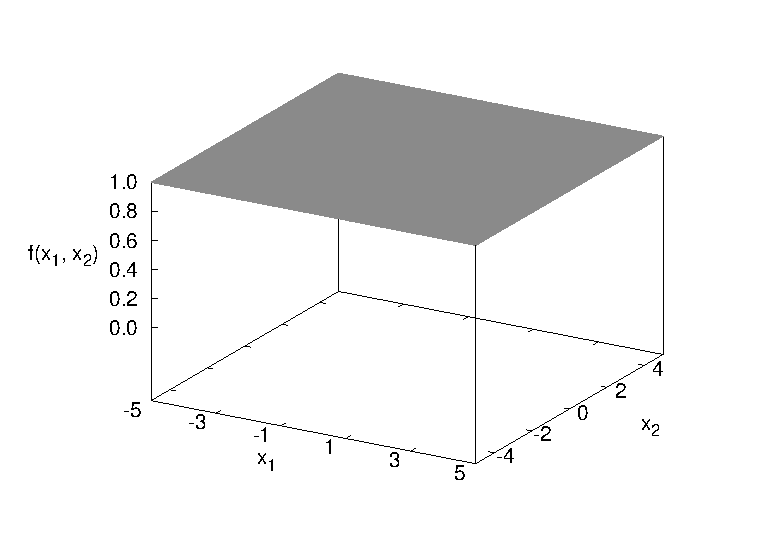
\includegraphics[width=0.25\linewidth]{flat}%
\label{figFlat}}
\subfloat[Inverted Almost-flat]{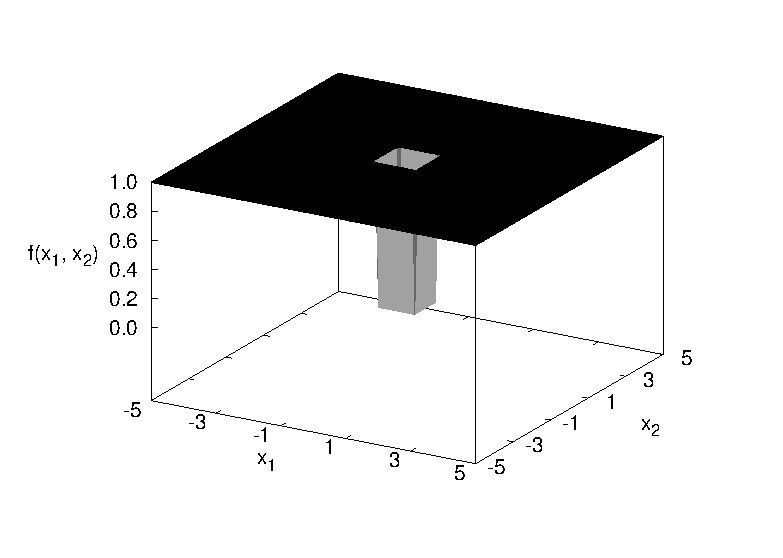
\includegraphics[width=0.25\linewidth]{almostFlat}%
\label{figAlmostFlat}}
\subfloat[Inverted Table]{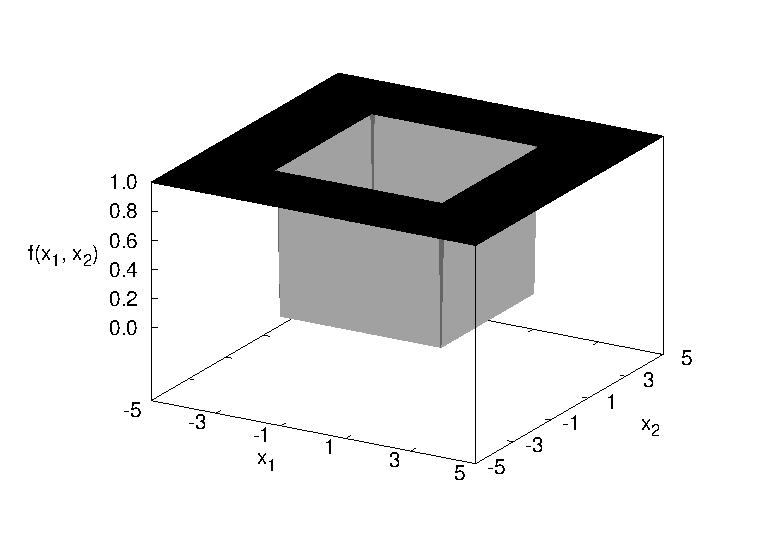
\includegraphics[width=0.25\linewidth]{table}%
\label{figTable}}
\subfloat[Easom]{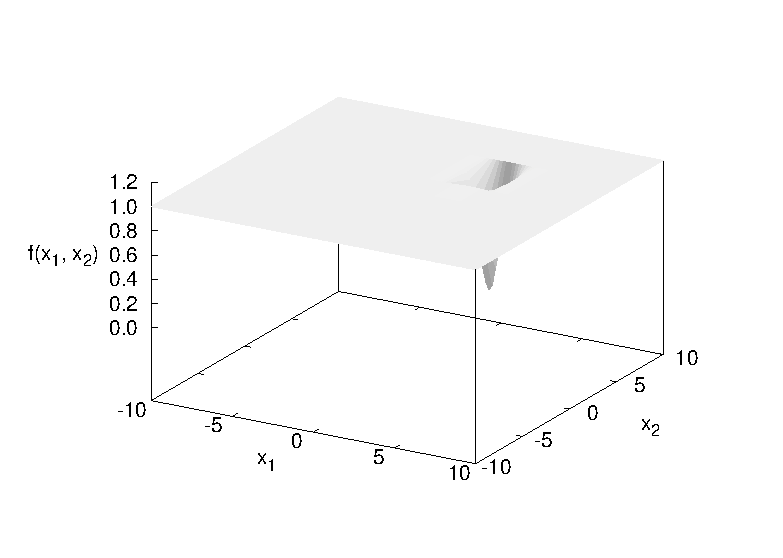
\includegraphics[width=0.25\linewidth]{easom}%
\label{figEasom}}

\subfloat[Step 2]{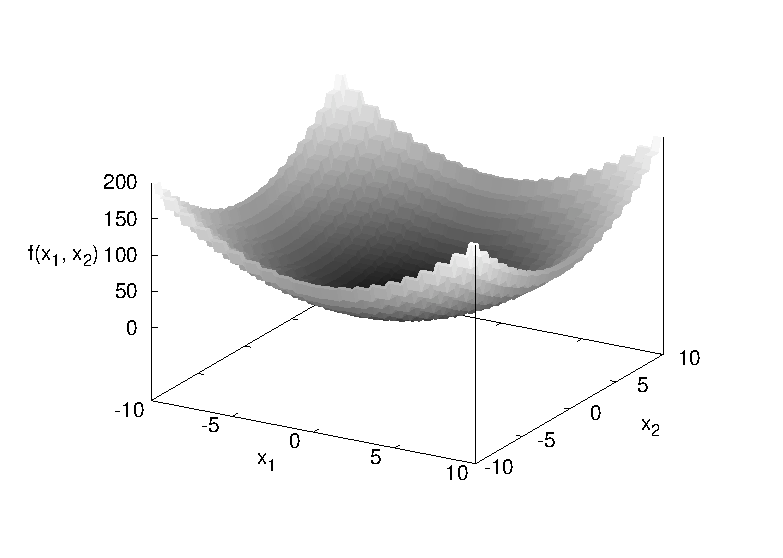
\includegraphics[width=0.25\linewidth]{step2}%
\label{figStep2}}
\subfloat[Step 1]{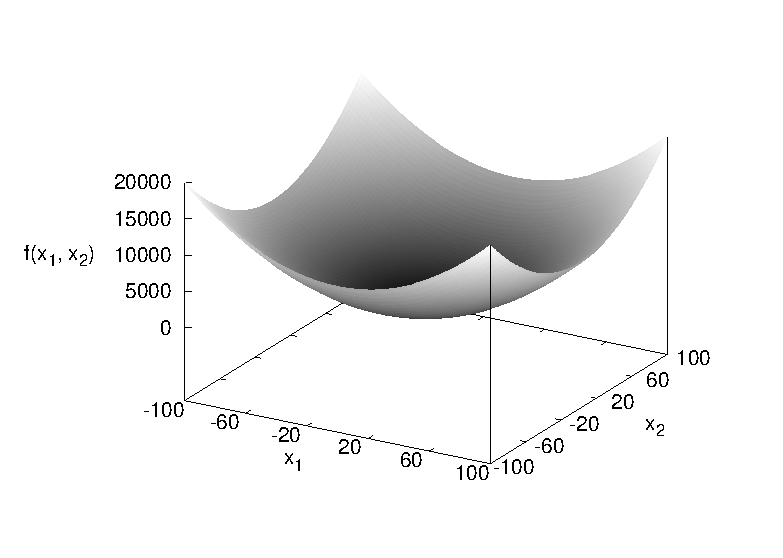
\includegraphics[width=0.25\linewidth]{step1}%
\label{figStep1}}
\subfloat[Absolute Value]{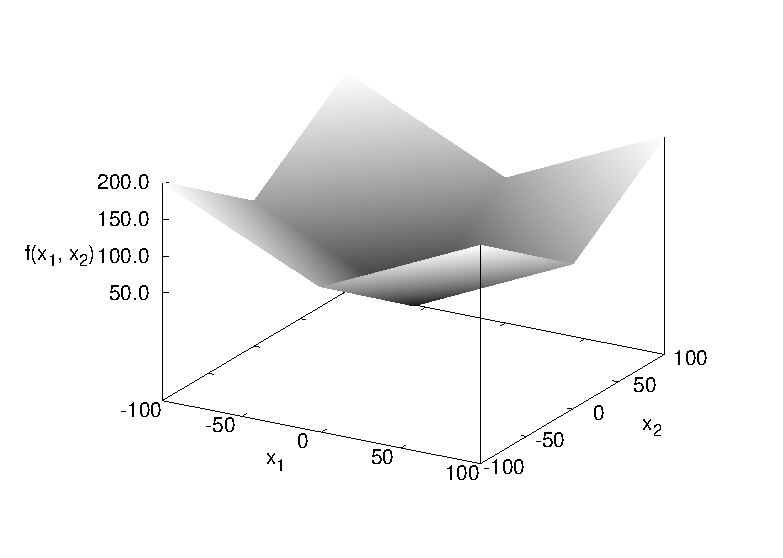
\includegraphics[width=0.25\linewidth]{absoluteValue}%
\label{figAbsoluteValue}}

\caption{Surface plots of two-dimensional benchmark problems, ranked according to the observed degree of neutrality}
\label{figVisBenchmark}
\end{figure*}

\subsection{Approach}
\label{visualApproach}
Both measures were initially applied to the benchmarks for dimensions $n=2$ to see whether the measures ranked the functions as expected. The measures were then applied on the same problems (excluding $f_{\text{Ea}}$) with increasing dimensions. Since the behaviour of most problems are not well understood for $n>2$, only the relative measure values could be used to determine whether the proposed measures performed as expected. That is, the same rank for the functions must be maintained for increasing values of $n$. Experiments were conducted as follows:

\begin{itemize}
	\item Algorithm \ref{algNeutralityMeasure} was applied 30 independent times for each measure, to each of the benchmark problems for $n=2$, to account for the stochastic nature of the sampling algorithm. From the 30 measurements, the averages and standard deviations were obtained. This was repeated for dimensions 3, 4, 5, 10 and 15.
	\item \citet{malan2014progressive} suggest the ideal number of walks to perform is equal to $2^n$, the number of starting zones, but they also note that it is infeasible. The number of walks were therefore set one order of magnitude greater than the dimension of the problem. That is $10n$.
	\item The step ratio is used to calculate the actual algorithm parameter, \textit{stepSize}, expressed as a proportion of the domain of the problem. Initial simulations showed that small step ratios $\le 0.01$ produced walks with little variability, progressing almost linearly through the landscape. The step ratio, and ultimately step size, cannot however be made too large, because neighbourhood information would be lost and the landscape under-represented. A $\textit{stepRatio} = 0.02$ was used.
	\item For $\mathcal{M}_2$ to make sense, the walk cannot be significantly longer than the domain of the problem. This would render the length of any longest neutral sequence an inconsequential fraction of the walk length. $numSteps$ were therefore set to 200 such that the landscape would, on average, be traversed only once.
	\item $\epsilon$ was set to 1.000E-8, often used in optimisation competitions as an acceptable trade-off to the known minimum of an objective function.
\end{itemize}


\subsection{Results}
\label{visualResults}
Table \ref{tblStaticProblems2} shows the averages and standard deviations obtained for ${\mathcal{M}_1}$ and ${\mathcal{M}_2}$ for two dimensions. The results establish that both measures are in agreement with the rank that was assigned to the problems. The measures appear to be consistent from the low standard deviation values which are frequently in the order of $10^{-3}$. As expected, $f_{\textit{St}_2}$ exhibited neutrality 3 orders of magnitude greater than its zoomed-out counterpart. $f_{\text{IA}}$ and 	$f_{\text{IT}}$ have similar values for ${\mathcal{M}_1}$. The two functions both have roughly the same level of neutrality present since both are completely flat apart from the 4 edges that walks would have to cross. The area covered by these edges are larger for $f_{\text{IT}}$, which would imply that a progressive walk would encounter these steep gradients more frequently, resulting is fewer neutral structures. However, the larger difference in measurements when using ${\mathcal{M}_2}$ on $f_{\text{IT}}$ and $f_{\text{IA}}$ can be explained by realising that the narrower protrusion in $f_{\text{IA}}$ would account for very large surrounding neutral regions, while the protrusion in $f_{\text{IT}}$ divides the space of neutral regions roughly in half, overall producing smaller regions. 

The values for the extreme cases of $f_{\text{Fl}}$ and $f_{\text{AV}}$ confirm that the measures correctly identify problems that are entirely flat and those that have no flat regions. Interestingly, ${\mathcal{M}_2}$, which indicates the size of neutral regions in the landscape, differs by 2 orders of magnitude between  $f_{\textit{St}_2}$ and  $f_{\textit{St}_1}$. This makes sense since we zoomed in by 2 orders of magnitude, thus increasing the size of all the steps in the landscape by the same amount. This is also roughly the case for ${\mathcal{M}_1}$

\begin{table}[!t] 
	\renewcommand{\arraystretch}{1.3}
	\caption{Averages and standard deviations of ${\mathcal{M}_1}$ and ${\mathcal{M}_2}$ for dimensions $n = 2$, on problems summarised in Table~\ref{functionBenchmarks}, in decreasing order}
	\label{tblStaticProblems2}
	\centering
	\begin{tabular}{|l|c|c|}
		\hline
		\textbf{Problem}					& ${\mathcal{M}_1}$ & ${\mathcal{M}_2}$ \\ \hline				
		$f_{\text{Fl}}$			& 1.000E+0 $\pm$ 0.000E+0 & 1.000E+0 $\pm$ 0.000E+0 \\
		$f_{\text{IA}}$			& 9.930E-1 $\pm$ 4.401E-3 & 9.930E-1 $\pm$ 4.401E-3 \\
		$f_{\text{IT}}$ 		& 9.596E-1 $\pm$ 1.597E-3 & 3.902E-1 $\pm$ 3.678E-2 \\
		$f_{\text{Ea}}$ 		& 8.443E-1 $\pm$ 1.848E-2 & 6.184E-1 $\pm$ 3.386E-2 \\
		$f_{\textit{St}_2}$ 	& 3.623E-1 $\pm$ 8.751E-3 & 2.434E-2 $\pm$ 1.813E-3 \\
		$f_{\textit{St}_1}$ 	& 1.843E-4 $\pm$ 2.463E-4 & 1.675E-4 $\pm$ 3.321E-4 \\
		$f_{\text{AV}}$			& 0.000E+0 $\pm$ 0.000E+0 & 0.000E+0 $\pm$ 0.000E+0 \\  \hline		
	\end{tabular}
\end{table}

Tables \ref{tblStaticProblemsNM1} and \ref{tblStaticProblemsNM2} show the values for measures ${\mathcal{M}_1}$ and ${\mathcal{M}_2}$ on problems whose dimensions were scaled. It is evident from both tables that the same order established in two dimensions are preserved across the other dimensions (as indicated by the colour coding). The measures maintain the same level of consistency as in two dimensions. It is worth noting the tendencies for both measures, on all problems, to gravitate to 0 or 1 as the dimensions increase (see figure \ref{figNeutralityVsDimensions}). This behaviour was thought to be associated with the insensitivity of algorithm parameters such as the \textit{stepSize} or perhaps the number of walks, but experiments that were repeated with absurd values that would be computationally infeasible in practice showed that, although more accurate, the measures presented the same tendencies. For reference, the number of walks were set to $2^n$ and \textit{numSteps} for ${\mathcal{M}_1}$ was set to 2000 when the behaviour was still apparent. It can therefore be concluded that the behaviour is either due to neutrality only appearing in a subset of the dimensions, for some problems, as dimensions increase, or the degree of neutrality increases for some problems as they are stretched out in higher dimensions. In both cases the behaviour is due to some change in the fitness landscape in higher dimensions.

\begin{table*}[!t]
	
	\centering
		\renewcommand{\arraystretch}{1.3}
	\caption{Averages and standard deviations of ${\mathcal{M}_1}$ for increasing dimensions, $n$, on scalable problems from Table~\ref{functionBenchmarks}. Ranking is indicated by shades of grey, with darker shades corresponding to higher values for ${\mathcal{M}_1}$}
	\label{tblStaticProblemsNM1}
	\begin{tabular}{|l|c|c|c|c|c|}
		\hline
		& \multicolumn{5}{c|}{\textbf{${\mathcal{M}_1}$ for Respective Dimensions}}\\ \cline{2-6} 
		\textbf{Problem}  & 3                                                                      & 4                                                                      & 5                                                                      & 10                                                                     & 15                                                                     \\ \hline
		$f_{\text{Fl}}$     & \cellcolor[HTML]{343434}{\color[HTML]{FFFFFF} 1.000E+0 $\pm$ 0.000E+0} & \cellcolor[HTML]{343434}{\color[HTML]{FFFFFF} 1.000E+0 $\pm$ 0.000E+0} & \cellcolor[HTML]{343434}{\color[HTML]{FFFFFF} 1.000E+0 $\pm$ 0.000E+0} & \cellcolor[HTML]{343434}{\color[HTML]{FFFFFF} 1.000E+0 $\pm$ 0.000E+0} & \cellcolor[HTML]{343434}{\color[HTML]{FFFFFF} 1.000E+0 $\pm$ 0.000E+0} \\
		$f_{\text{IA}}$     & \cellcolor[HTML]{656565}{\color[HTML]{FFFFFF} 9.988E-1 $\pm$ 1.646E-3} & \cellcolor[HTML]{656565}{\color[HTML]{FFFFFF} 9.997E-1 $\pm$ 1.085E-3} & \cellcolor[HTML]{656565}{\color[HTML]{FFFFFF} 9.999E-1 $\pm$ 5.100E-4} & \cellcolor[HTML]{343434}{\color[HTML]{FFFFFF} 1.000E+0 $\pm$ 0.000E+0} & \cellcolor[HTML]{343434}{\color[HTML]{FFFFFF} 1.000E+0 $\pm$ 0.000E+0} \\
		$f_{\text{IT}}$     & \cellcolor[HTML]{9B9B9B}{\color[HTML]{FFFFFF} 9.638E-1 $\pm$ 2.733E-3} & \cellcolor[HTML]{9B9B9B}{\color[HTML]{FFFFFF} 9.670E-1 $\pm$ 4.079E-3} & \cellcolor[HTML]{9B9B9B}{\color[HTML]{FFFFFF} 9.696E-1 $\pm$ 4.525E-3} & \cellcolor[HTML]{656565}{\color[HTML]{FFFFFF} 9.784E-1 $\pm$ 5.368E-3} & \cellcolor[HTML]{656565}{\color[HTML]{FFFFFF} 9.842E-1 $\pm$ 5.424E-3} \\
		$f_{\textit{St}_2}$ & \cellcolor[HTML]{C0C0C0}2.218E-1 $\pm$ 8.046E-3                        & \cellcolor[HTML]{C0C0C0}1.382E-1 $\pm$ 7.509E-3                        & \cellcolor[HTML]{DFDFDF}8.817E-2 $\pm$ 6.799E-3                        & \cellcolor[HTML]{DFDFDF}9.732E-3 $\pm$ 1.713E-3                        & \cellcolor[HTML]{DFDFDF}1.776E-3 $\pm$ 9.583E-4                        \\
		$f_{\textit{St}_1}$ & \cellcolor[HTML]{DFDFDF}1.675E-5 $\pm$ 9.175E-5                        & 0.000E+0 $\pm$ 0.000E+0                                                & 0.000E+0 $\pm$ 0.000E+0                                                & 0.000E+0 $\pm$ 0.000E+0                                                & 0.000E+0 $\pm$ 0.000E+0                                                \\
		$f_{\text{AV}}$     & 0.000E+0 $\pm$ 0.000E+0                                                & 0.000E+0 $\pm$ 0.000E+0                                                & 0.000E+0 $\pm$ 0.000E+0                                                & 0.000E+0 $\pm$ 0.000E+0                                                & 0.000E+0 $\pm$ 0.000E+0                                                \\ \hline
	\end{tabular}
\end{table*}


\begin{table*}[]
	\centering
	\renewcommand{\arraystretch}{1.3}
	\caption{Averages and standard deviations of ${\mathcal{M}_2}$ for increasing dimensions, $n$, on scalable problems from Table~\ref{functionBenchmarks}. Ranking is indicated by shades of grey, with darker shades corresponding to higher values for ${\mathcal{M}_2}$}
	\label{tblStaticProblemsNM2}
	\begin{tabular}{|l|c|c|c|c|c|}
		\hline
		& \multicolumn{5}{c|}{\textbf{${\mathcal{M}_2}$ for Respective Dimensions}}\\ \cline{2-6} 
		\textbf{Problem}  & 3                                                                      & 4                                                                      & 5                                                                      & 10                                                                     & 15                                                                     \\ \hline
		$f_{\text{Fl}}$     & \cellcolor[HTML]{343434}{\color[HTML]{FFFFFF} 1.000E+0 $\pm$ 0.000E+0} & \cellcolor[HTML]{343434}{\color[HTML]{FFFFFF} 1.000E+0 $\pm$ 0.000E+0} & \cellcolor[HTML]{343434}{\color[HTML]{FFFFFF} 1.000E+0 $\pm$ 0.000E+0} & \cellcolor[HTML]{343434}{\color[HTML]{FFFFFF} 1.000E+0 $\pm$ 0.000E+0} & \cellcolor[HTML]{343434}{\color[HTML]{FFFFFF} 1.000E+0 $\pm$ 0.000E+0} \\
		$f_{\text{IA}}$     & \cellcolor[HTML]{656565}{\color[HTML]{FFFFFF} 9.765E-1 $\pm$ 2.790E-2} & \cellcolor[HTML]{656565}{\color[HTML]{FFFFFF} 9.949E-1 $\pm$ 1.439E-2} & \cellcolor[HTML]{656565}{\color[HTML]{FFFFFF} 9.982E-1 $\pm$ 1.000E-2} & \cellcolor[HTML]{343434}{\color[HTML]{FFFFFF} 1.000E+0 $\pm$ 0.000E+0} & \cellcolor[HTML]{343434}{\color[HTML]{FFFFFF} 1.000E+0 $\pm$ 0.000E+0} \\
		$f_{\text{IT}}$     & \cellcolor[HTML]{9B9B9B}{\color[HTML]{FFFFFF} 4.759E-1 $\pm$ 5.393E-2} & \cellcolor[HTML]{9B9B9B}{\color[HTML]{FFFFFF} 5.389E-1 $\pm$ 8.194E-2} & \cellcolor[HTML]{9B9B9B}{\color[HTML]{FFFFFF} 5.751E-1 $\pm$ 8.100E-2} & \cellcolor[HTML]{9B9B9B}{\color[HTML]{FFFFFF} 7.397E-1 $\pm$ 7.721E-2} & \cellcolor[HTML]{656565}{\color[HTML]{FFFFFF} 8.212E-1 $\pm$ 5.069E-2} \\
		$f_{\textit{St}_2}$ & \cellcolor[HTML]{C0C0C0}1.754E-2 $\pm$ 1.348E-3                        & \cellcolor[HTML]{C0C0C0}1.369E-2 $\pm$ 1.148E-3                        & \cellcolor[HTML]{C0C0C0}1.095E-2 $\pm$ 8.793E-4                        & \cellcolor[HTML]{DFDFDF}5.025E-3 $\pm$ 8.950E-4                        & \cellcolor[HTML]{DFDFDF}1.608E-3 $\pm$ 7.962E-4                        \\
		$f_{\textit{St}_1}$ & \cellcolor[HTML]{FFFFFF}0.000E+0 $\pm$ 0.000E+0                        & 0.000E+0 $\pm$ 0.000E+0                                                & 0.000E+0 $\pm$ 0.000E+0                                                & 0.000E+0 $\pm$ 0.000E+0                                                & 0.000E+0 $\pm$ 0.000E+0                                                \\
		$f_{\text{AV}}$     & 0.000E+0 $\pm$ 0.000E+0                                                & 0.000E+0 $\pm$ 0.000E+0                                                & 0.000E+0 $\pm$ 0.000E+0                                                & 0.000E+0 $\pm$ 0.000E+0                                                & 0.000E+0 $\pm$ 0.000E+0                                                \\ \hline
	\end{tabular}
\end{table*}

\begin{figure}[!ht]
	\centering
	\subfloat[]{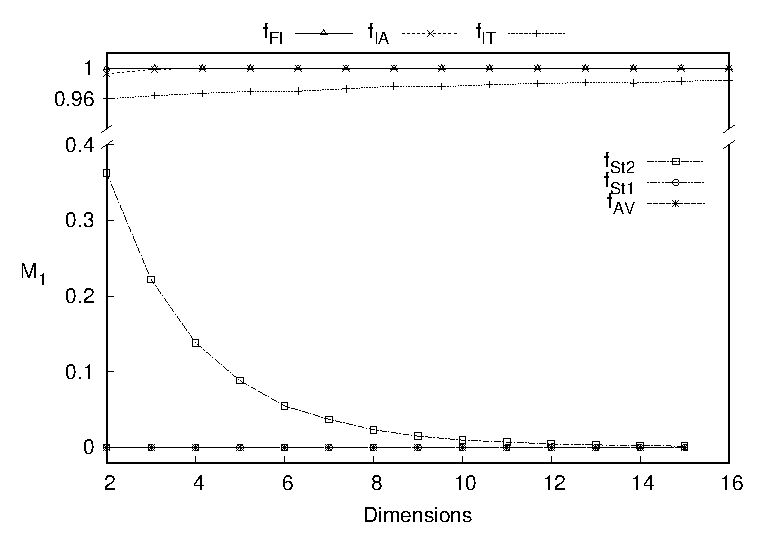
\includegraphics[width=\linewidth]{neutralityVsDimensionsM1}}%
	\label{figNeutralityVsDimensionsM1}	
		
	\subfloat[]{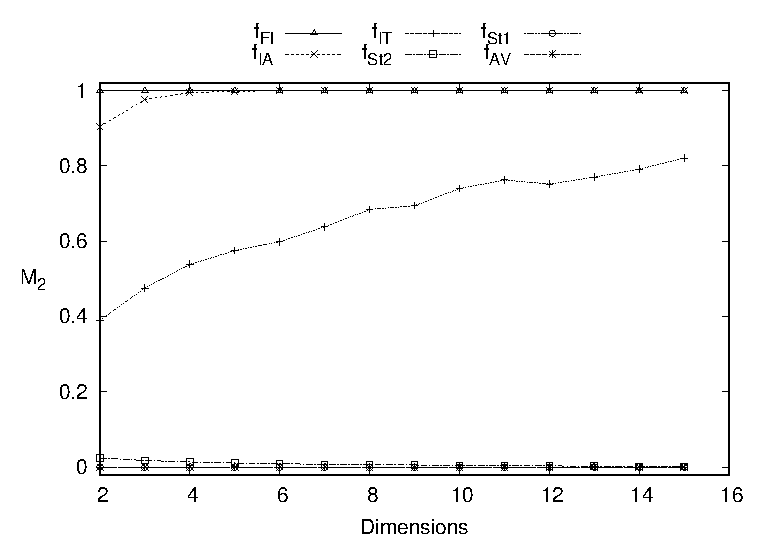
\includegraphics[width=\linewidth]{neutralityVsDimensionsM2}}%
	\label{figNeutralityVsDimensionsM2}	
	\caption{Degree of neutrality measured versus dimensionality on problems from Table~\ref{functionBenchmarks} using (a) ${\mathcal{M}_1}$ and (b) ${\mathcal{M}_2}$ }
	\label{figNeutralityVsDimensions}
\end{figure}

Figure \ref{figStep2Sampled} shows a projection of the $f_{\textit{St}_2}$ landscape on the $x_1x_2$-plane, together with a sample of the landscape resulting from a single run of the algorithm. This illustrates that, at least in two dimensions, the sample of the surface exhibits good variability and doesn't neglect large parts of the search space.

\begin{figure}[!ht]
	\centering
	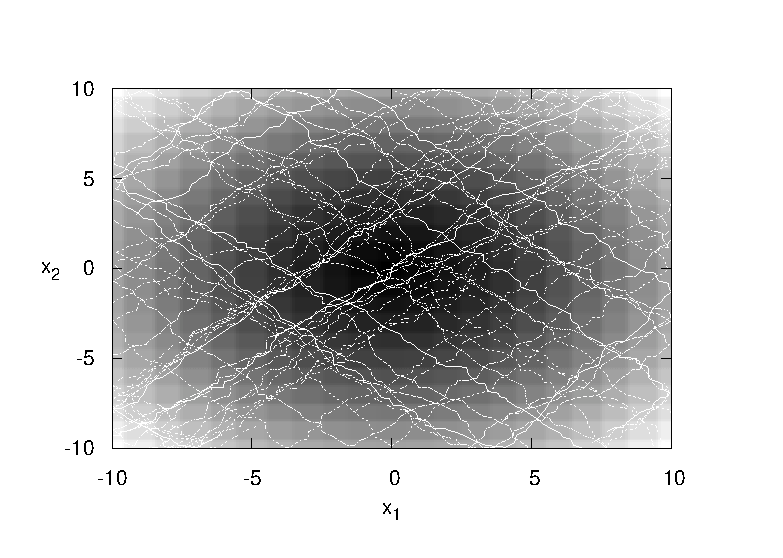
\includegraphics[width=\linewidth]{step2Sampled}%
		
	\caption{A map of $f_{\textit{St}_2}$. The various dashed lines represent an archetypal sample of the landscape, performed using algorithm \ref{algProgRandomWalk} with $10n$ walks, one walk every ${2^n/10n}_{\text{th}}$ starting zone. Step sizes were capped at $2\%$ of the domain and $200$ steps for each walk.}
	\label{figStep2Sampled}
\end{figure}

\section{Application to Neural Network Error Landscapes}
\label{nnELApplication}
One area of application for the proposed neutrality measures, is the study of NN error landscapes. As noted in section \ref{backgroundNNEL}, it has long been thought that the NN error surface consists of large neutral regions such as plateaus and ridges. This section of the paper applies ${\mathcal{M}_1}$ and ${\mathcal{M}_2}$ to some well known benchmark datasets for classification.

\subsection{Benchmark Problems}
\label{nnBenchmarks}
For this phase of the study, apart from the XOR problem, benchmarks of varying complexity were obtained from the UCI Machine Learning Repository \cite{Lichman2013}. Optimal NN architectures for each benchmark were employed, summarised in table \ref{tblNNBenchmarks}. The study was limited to feed-forward NNs, using the sigmoid activation function and the mean squared error (MSE) loss function.

\begin{table}[!t] 
	\renewcommand{\arraystretch}{1.3}
	\caption{Benchmark datasets and their corresponding optimal three-layer NN architecture, in the format \#inputUnits-\#hiddenUnits-\#outputUnits}
	\label{tblNNBenchmarks}
	\centering
	\begin{tabular}{|l|l|}
		\hline
		\textbf{Dataset}		& \textbf{Architecture} \\ \hline				
		XOR									&  2-2-1		\\
		Iris								&  4-4-3 \cite{gupta1998weight}		\\
		Diabetes							&  8-6-1 \cite{carvalho2006particle}			\\
		Glass Identification (Glass)		&  9-9-6 \cite{gupta1998weight}			\\
		Breast Cancer Wisconsin (Cancer)	&  30-6-1 \cite{carvalho2006particle}		\\
		Heart Disease (Heart)				&  32-6-1 \cite{carvalho2006particle}	\\ \hline		
	\end{tabular}
\end{table}

All pattern inputs and outputs in the benchmark suite were scaled to the active domain and range of the Sigmoid activation function, $[-1,1]$ and $[0.1,0.9]$, respectively.
	
\subsection{Approach}
\label{nnApproach}
The parameters of the experiment were similar to that in section \ref{visualAnalysis}, except for a few minor deviations.

\begin{itemize}
	\item Algorithm \ref{algNeutralityMeasure} was again applied 30 independent times for each measure, to each of the benchmark problems in table \ref{tblNNBenchmarks}. This was done for various values of $x^{\text{max}}$, with the domain of the sample in all dimensions defined as $[-x^{\text{max}}, x^{\text{max}}]$.
	\item Sampling the NN problems were prohibitively expensive, and therefore the number of walks was restricted to $2n$.
	\item All other parameters were the same.
\end{itemize}

\subsection{Results}
\label{nnResults}



\begin{figure}[!t]
	\centering
	\subfloat[]{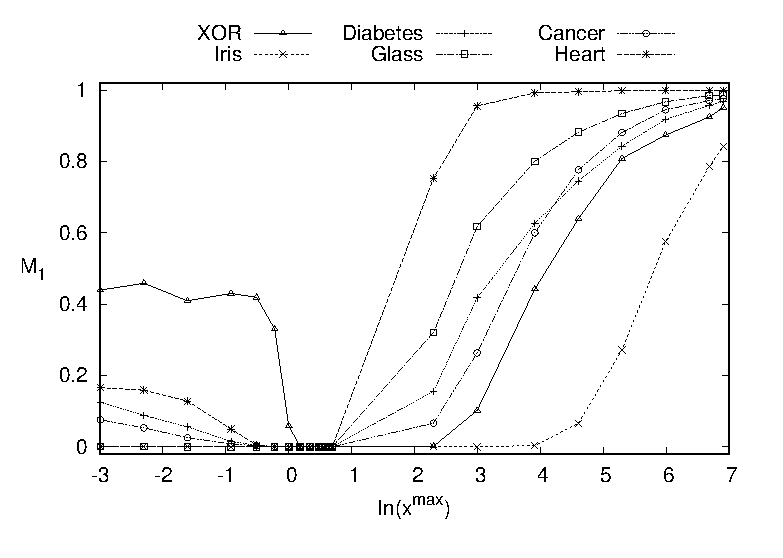
\includegraphics[width=\linewidth]{nnNeutralityVsDomainM1}}%
	\label{figNNM1}	
	
	\subfloat[]{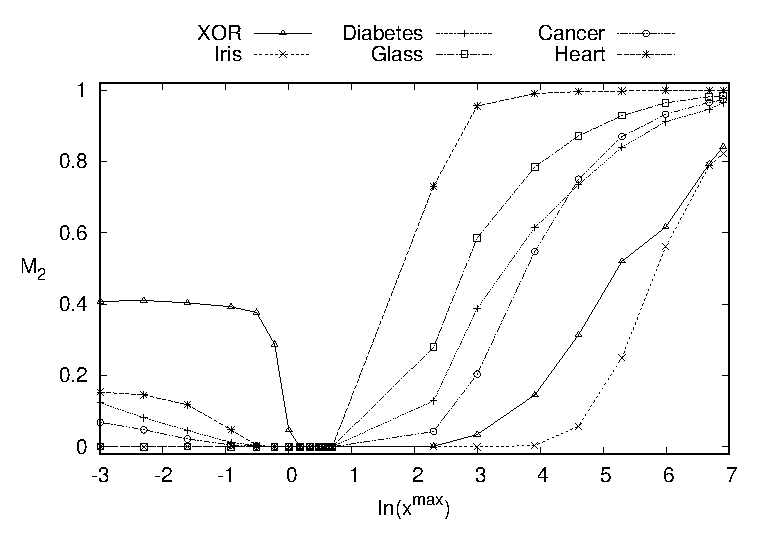
\includegraphics[width=\linewidth]{nnNeutralityVsDomainM2}}%
	\label{figNNM2}	
	\caption{Degree of neutrality measured versus the sample bounds on NN benchmarks in section \ref{nnBenchmarks} using (a) ${\mathcal{M}_1}$ and (b) ${\mathcal{M}_2}$. The domain of each dimension, $x_i$, has been fixed to $[-x^{\text{max}}, x^{\text{max}}]$}
	\label{figNNNeutralityVsDomain}
\end{figure}

\section{Conclusion}
In this paper, it was shown how two complementary measures of neutrality, ${\mathcal{M}_1}$ and ${\mathcal{M}_2}$, based on a progressive random walk sample of the landscape, can successfully be used to characterise the search landscape in terms of the presence and size of neutral regions. The measures were tested on a relatively small set of benchmark functions that can be expanded in future research. The definition of the neutrality measures also allow for various levels of sensitivity to be adjusted, optimal values of which have yet to be determined empirically in an extensive study. $\epsilon$ can be increased in cases where the detection of near-neutrality is important. 

${\mathcal{M}_1}$ and ${\mathcal{M}_2}$ have also helped confirm the saturation-induced neutrality present in NN error landscapes. The results were however in disagreement with other studies that have suggested that regions around the origin are often neutral when using a symmetric activation function \cite{lecun2012efficient}, but further investigation is necessary on a larger benchmark suite and more combinations of loss- and activation functions to determine if the phenomenon does indeed occur.

% An example of a floating figure using the graphicx package.
% Note that \label must occur AFTER (or within) \caption.
% For figures, \caption should occur after the \includegraphics.
% Note that IEEEtran v1.7 and later has special internal code that
% is designed to preserve the operation of \label within \caption
% even when the captionsoff option is in effect. However, because
% of issues like this, it may be the safest practice to put all your
% \label just after \caption rather than within \caption{}.
%
% Reminder: the "draftcls" or "draftclsnofoot", not "draft", class
% option should be used if it is desired that the figures are to be
% displayed while in draft mode.
%
%\begin{figure}[!t]
%\centering
%\includegraphics[width=2.5in]{myfigure}
% where an .eps filename suffix will be assumed under latex, 
% and a .pdf suffix will be assumed for pdflatex; or what has been declared
% via \DeclareGraphicsExtensions.
%\caption{Simulation results for the network.}
%\label{fig_sim}
%\end{figure}

% Note that the IEEE typically puts floats only at the top, even when this
% results in a large percentage of a column being occupied by floats.


% An example of a double column floating figure using two subfigures.
% (The subfig.sty package must be loaded for this to work.)
% The subfigure \label commands are set within each subfloat command,
% and the \label for the overall figure must come after \caption.
% \hfil is used as a separator to get equal spacing.
% Watch out that the combined width of all the subfigures on a 
% line do not exceed the text width or a line break will occur.
%
%\begin{figure*}[!t]
%\centering
%\subfloat[Case I]{\includegraphics[width=2.5in]{box}%
%\label{fig_first_case}}
%\hfil
%\subfloat[Case II]{\includegraphics[width=2.5in]{box}%
%\label{fig_second_case}}
%\caption{Simulation results for the network.}
%\label{fig_sim}
%\end{figure*}
%
% Note that often IEEE papers with subfigures do not employ subfigure
% captions (using the optional argument to \subfloat[]), but instead will
% reference/describe all of them (a), (b), etc., within the main caption.
% Be aware that for subfig.sty to generate the (a), (b), etc., subfigure
% labels, the optional argument to \subfloat must be present. If a
% subcaption is not desired, just leave its contents blank,
% e.g., \subfloat[].


% An example of a floating table. Note that, for IEEE style tables, the
% \caption command should come BEFORE the table and, given that table
% captions serve much like titles, are usually capitalized except for words
% such as a, an, and, as, at, but, by, for, in, nor, of, on, or, the, to
% and up, which are usually not capitalized unless they are the first or
% last word of the caption. Table text will default to \footnotesize as
% the IEEE normally uses this smaller font for tables.
% The \label must come after \caption as always.
%
%\begin{table}[!t]
%% increase table row spacing, adjust to taste
%\renewcommand{\arraystretch}{1.3}
% if using array.sty, it might be a good idea to tweak the value of
% \extrarowheight as needed to properly center the text within the cells
%\caption{An Example of a Table}
%\label{table_example}
%\centering
%% Some packages, such as MDW tools, offer better commands for making tables
%% than the plain LaTeX2e tabular which is used here.
%\begin{tabular}{|c||c|}
%\hline
%One & Two\\
%\hline
%Three & Four\\
%\hline
%\end{tabular}
%\end{table}


% Note that the IEEE does not put floats in the very first column
% - or typically anywhere on the first page for that matter. Also,
% in-text middle ("here") positioning is typically not used, but it
% is allowed and encouraged for Computer Society conferences (but
% not Computer Society journals). Most IEEE journals/conferences use
% top floats exclusively. 
% Note that, LaTeX2e, unlike IEEE journals/conferences, places
% footnotes above bottom floats. This can be corrected via the
% \fnbelowfloat command of the stfloats package.

% trigger a \newpage just before the given reference
% number - used to balance the columns on the last page
% adjust value as needed - may need to be readjusted if
% the document is modified later
%\IEEEtriggeratref{8}
% The "triggered" command can be changed if desired:
%\IEEEtriggercmd{\enlargethispage{-5in}}

% references section

% \bibliography{Bibliography/bibliography}
% \bibliographystyle{IEEEtran}

\printbibliography

\end{document}


